
È stato utilizzato mUSE di Google (vedi Sezione~\ref{sec:use}), perchè si ipotizza che le frasi appartenenti allo stesso topic siano simili fra loro e di conseguenza anche i vettori risultanti dall'operazione di embedding saranno simili. Per verificare questa ipotesi è stato selezionato un campione {\tt random} di 5 frasi per ogni topic, è stato effettuato l'embed delle frasi e poi calcolato l'inner product degli embed. L'inner product è una tecnica molto semplice per comprendere la similarità tra due vettori. Il valore di similarità $s \in [0..1]$, dove $1$ indica frasi / vettori identiche / ci, $0$ indica completa dissimilarità, quindi più il valore è vicino a $1$ più le / i frasi / vettori sono simili.

Di seguito vengono mostrate le metrici di similarità ottenute dell'inner product. Si può notare che le matrici di similarità con i valori più alti sono:
\begin{itemize}
    \item politics (Fig.\ref{fig:mtrsim_p}): con valori che vanno da 0.63 a 1
    \item job (Fig.\ref{fig:mtrsim_j}): con valori che vanno da 0.72 a 1
\textbf{I restanti invece presentano valori di similarità molto più bassi.}

Infine, è stata realizzata una matrice che mette insieme le frasi scelte dai vari topic per valutare quanto le frasi appartenenti a diversi topic si somigliassero (differiscano tra loro in questo caso). Il risultato è mostrato in Fig.~\ref{fig:mtrsim_mix} dove si può notare che le celle colorate con toni chiari (valori superiori a 0.5) siano ottenute dalla intersezione di frasi appartenenti allo stesso topic, mentre, le celle colorate con toni scuri (valori inferiori al 0.5) siano date dell'inner product di frasi appartenenti a topic diversi.
\end{itemize}
\begin{figure}[h!t]
    \centering
    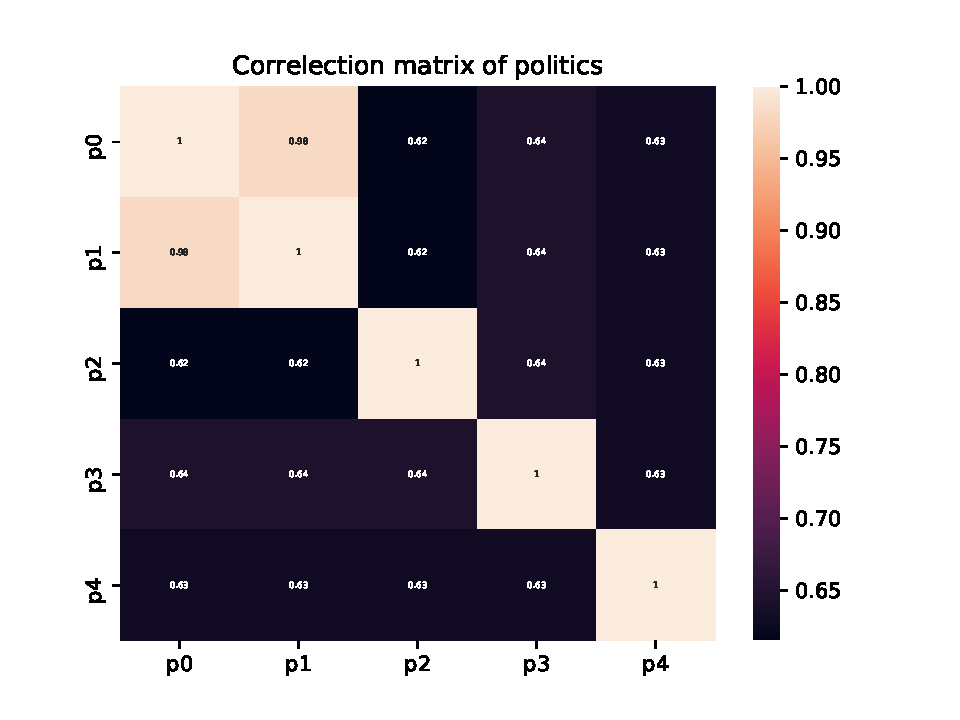
\includegraphics{Figure/simMatr/politics.pdf}
    \caption{matrici di similarità delle frasi appartenenti al topic politics}
    \label{fig:mtrsim_p}
\end{figure}
\FloatBarrier

\begin{figure}[h!t]
    \centering
    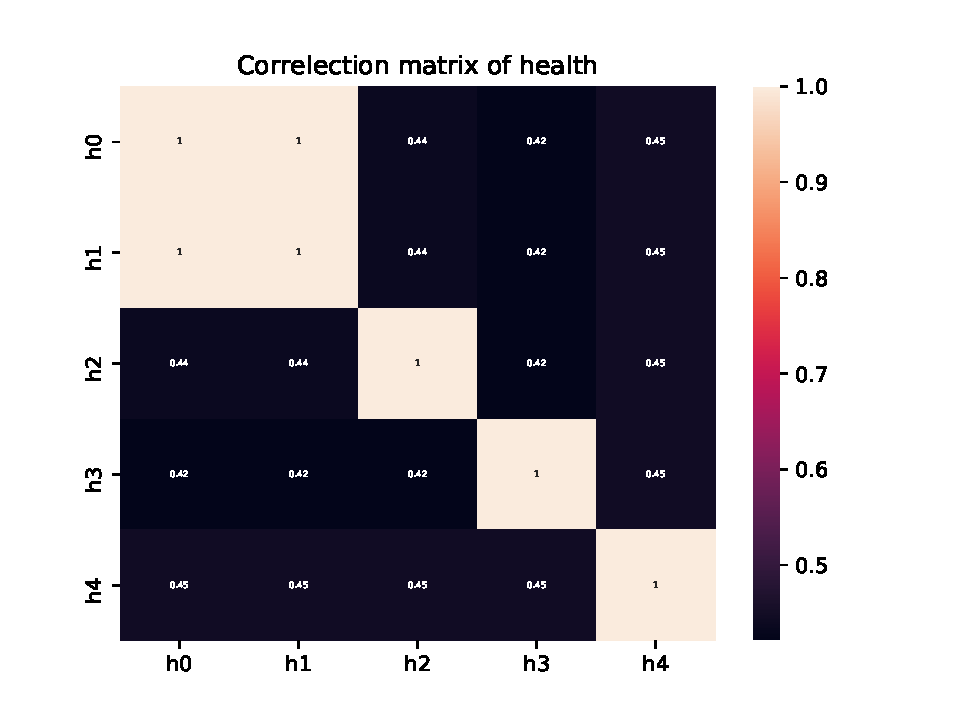
\includegraphics{Figure/simMatr/health.pdf}
    \caption{matrici di similarità delle frasi appartenenti al topic health}
    \label{fig:mtrsim_h}
\end{figure}
\FloatBarrier

\begin{figure}[h!t]
    \centering
    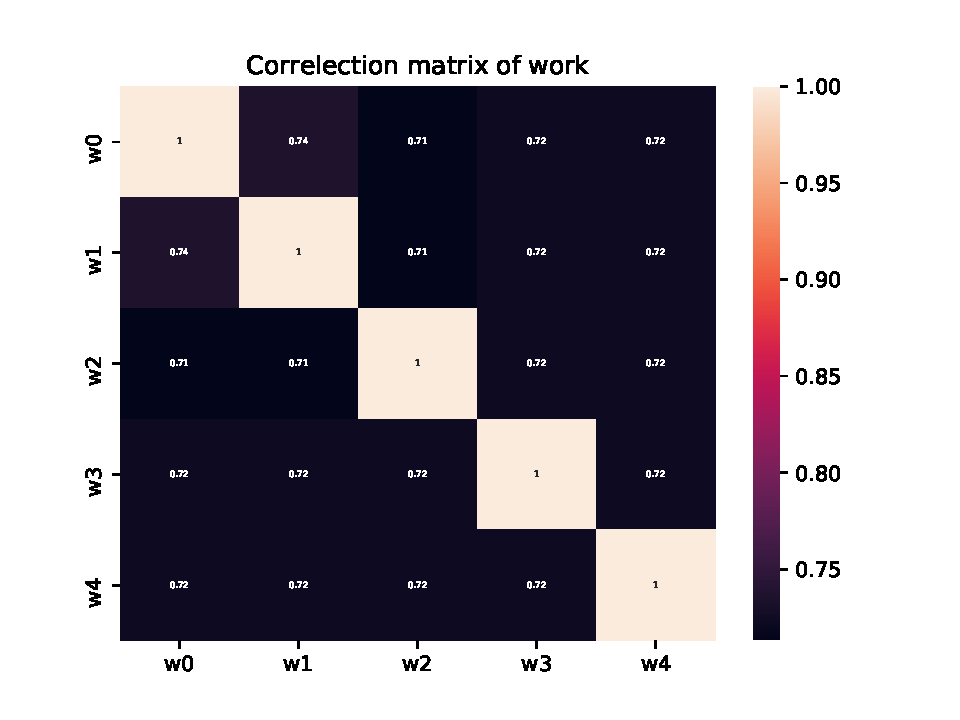
\includegraphics{Figure/simMatr/work.pdf}
    \caption{matrici di similarità delle frasi appartenenti al topic job}
    \label{fig:mtrsim_j}
\end{figure}
\FloatBarrier

\begin{figure}[h!t]
    \centering
    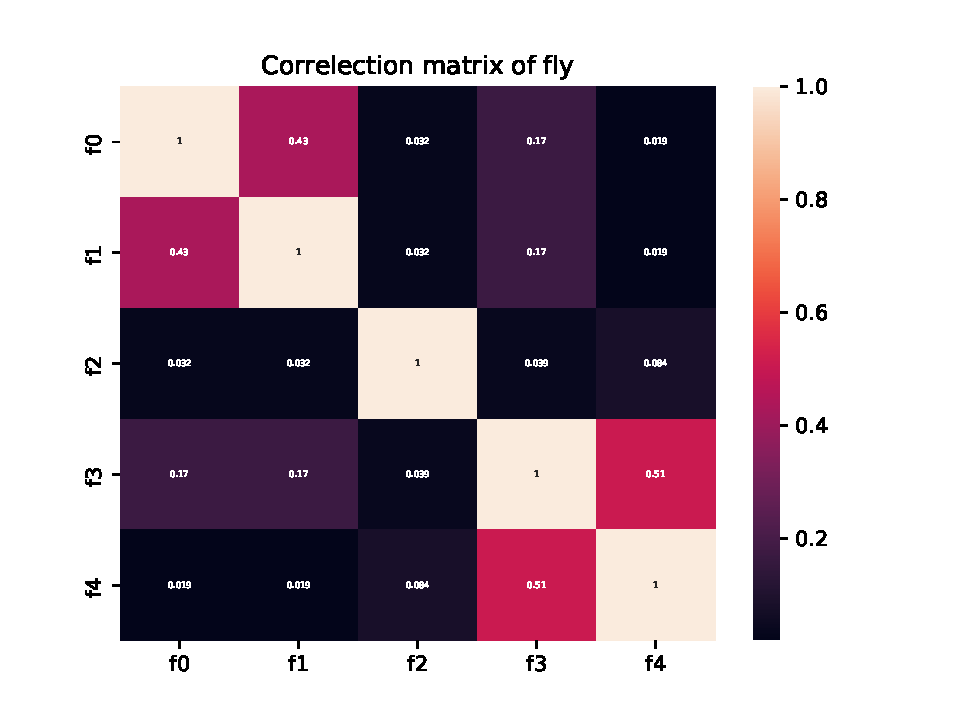
\includegraphics{Figure/simMatr/fly.pdf}
    \caption{matrici di similarità delle frasi appartenenti al topic travel}
    \label{fig:mtrsim_t}
\end{figure}
\FloatBarrier

\begin{figure}[h!t]
    \centering
    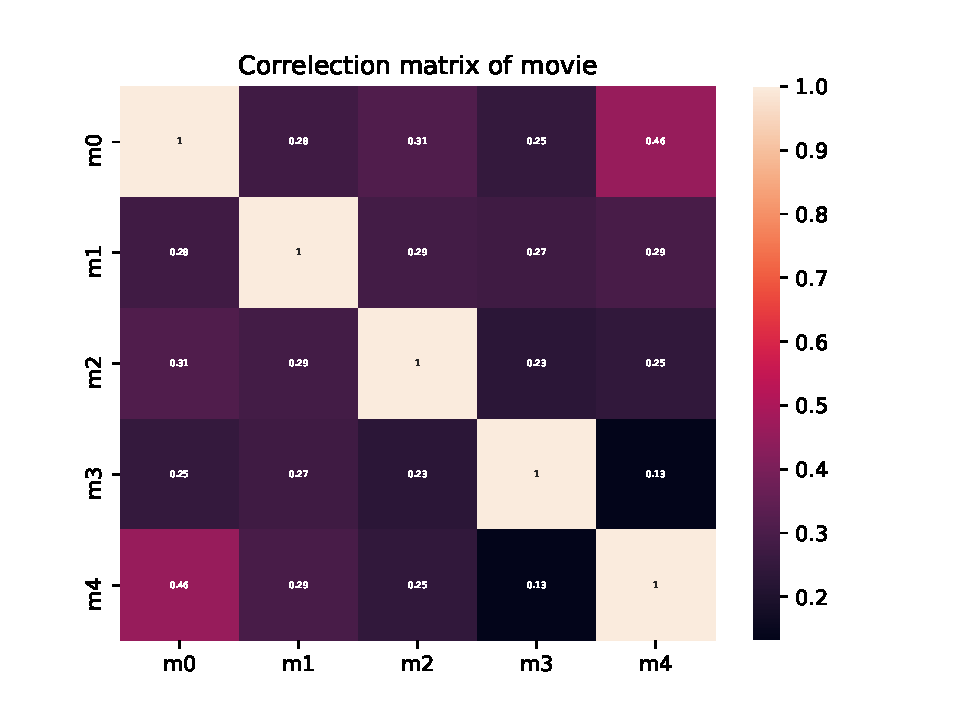
\includegraphics{Figure/simMatr/movie.pdf}
    \caption{matrici di similarità delle frasi appartenenti al topic general}
    \label{fig:mtrsim_g}
\end{figure}
\FloatBarrier

\begin{figure}[h!t]
    \centering
    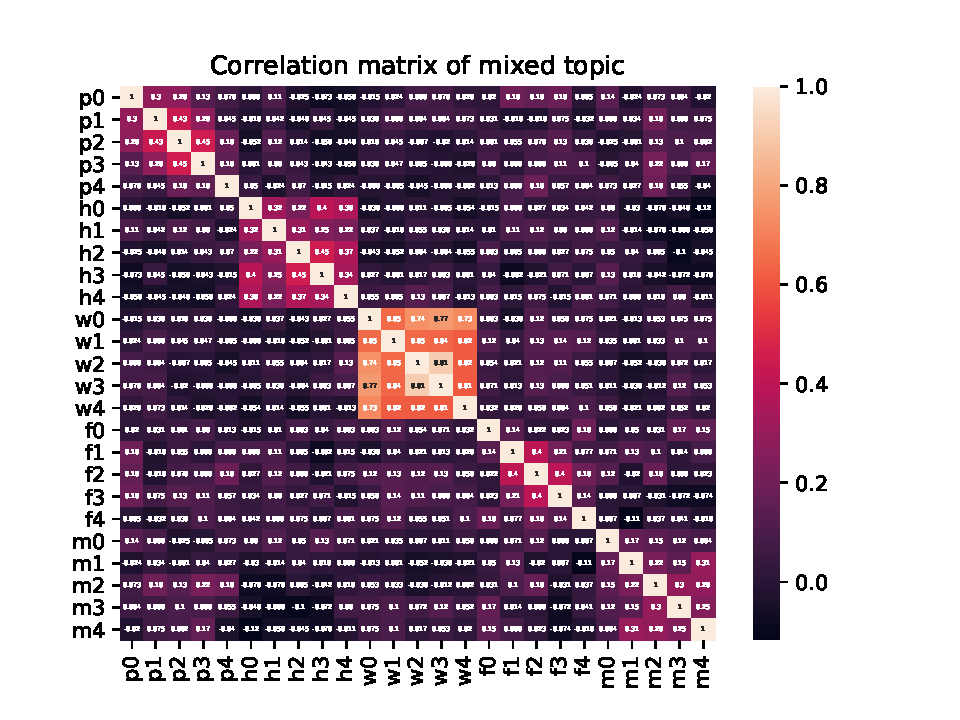
\includegraphics{Figure/simMatr/mixed.pdf}
    \caption{matrici di similarità delle frasi appartenenti ai diversi topic}
    \label{fig:mtrsim_mix}
\end{figure}
\FloatBarrier
